%!TEX encoding = UTF-8 Unicode
\documentclass[runningheads]{llncs}

%% ── 宏包 ─────────────────────────────────────────────────────────────────
\usepackage{booktabs}
\usepackage{multirow}
\usepackage{makecell}
\usepackage{graphicx}
\usepackage{subcaption}
\usepackage{amsmath,amssymb,amsfonts}
\usepackage{algorithm}
\usepackage{algpseudocode}
\usepackage{listings}
\usepackage{xcolor}
\usepackage{microtype}
\usepackage{enumitem}
\usepackage{tikz}
\usepackage{pgfplots}
\pgfplotsset{compat=1.18}
\usepackage{hyperref}
\usepackage{ctex}
\usepackage{fontspec}

%% TikZ 库用于激励示例图
\usetikzlibrary{shapes.geometric,arrows.meta,positioning,fit,backgrounds}

%% ── 代码列表样式 ───────────────────────────────────────────────────────────
\lstset{
  basicstyle=\ttfamily\scriptsize,
  breaklines=true,
  frame=single,
  numbers=left, numberstyle=\tiny,
  keywordstyle=\color{blue!70!black}\bfseries,
  commentstyle=\color{gray},
  stringstyle=\color{teal},
}

% 注意：LLNCS 已定义 \problem 环境，无需重新定义
\begin{document}

\title{OASIS：面向基于成本的查询优化器的反馈驱动统计信息校正系统}

\author{作者姓名（审稿阶段隐去）}

\authorrunning{作者姓名（审稿阶段隐去）}

\institute{所属机构（审稿阶段隐去）\\
\email{redacted@review.org}}

\maketitle

\begin{abstract}
在大规模分析型数据库中，基于成本的优化器（CBO）的准确性严重依赖于列级统计信息的新鲜度。
在实际应用中，列统计信息仅通过昂贵的全表\texttt{ANALYZE}扫描进行刷新，通常每天或更低频率执行一次，
而表则持续经历DML工作负载——这造成了持久的\emph{陈旧性差距}，导致系统性的选择性估计错误、
次优的连接顺序选择以及可测量的查询性能下降。

本文提出\textbf{OASIS}（\textbf{O}nline \textbf{A}daptive \textbf{S}tatistics
\textbf{I}nference \textbf{S}ystem，在线自适应统计信息推理系统），一个面向列级\emph{统计信息校正}的反馈驱动框架。
与调整优化器提示或连接顺序的计划级反馈方法不同，
OASIS直接在CBO消费的统计信息表示上进行操作，
无需重新扫描表或修改查询引擎即可从查询执行观测中修复陈旧的列直方图。
它将每个校正实例编码为紧凑的、与模型无关的特征张量，
并支持可互换的校正策略，范围从无需训练的分析基线（Teacher）到在模拟派生的真实标签上训练的\emph{注意力池化MLP}，无需人工标注。
共享的特征表示与模型无关，允许在不改变系统接口的情况下升级校正后端。
该系统通过单一注入点以非侵入方式集成到现有统计信息管道中，CBO和执行引擎保持不变。

我们在不同强度的合成漂移场景、冷启动条件、敏感性分析和端到端基准测试中进行了全面的实验，
证明了OASIS显著优于陈旧统计信息，提高了选择性估计准确性。
\keywords{统计信息校正 \and 基数估计 \and 直方图校准 \and
统计信息陈旧性 \and 基于成本的优化器 \and 保序回归 \and
查询反馈 \and 机器学习 \and 在线学习}
\end{abstract}

%% ═══════════════════════════════════════════════════════════════════════════
\section{引言}
\label{sec:intro}
%% ═══════════════════════════════════════════════════════════════════════════

\paragraph{陈旧性问题。}
现代分析型查询引擎依赖列级直方图来估计谓词选择性，进而驱动连接顺序选择和算子算法选择。
列统计信息通过周期性的\texttt{ANALYZE}扫描进行刷新——这相当于一次完整的表扫描——操作成本高昂，
通常每天或更低频率执行。
与此同时，表持续接收插入、删除和更新操作。
结果是持久的\emph{陈旧性差距}：如图\ref{fig:motivating}所示，
CBO的选择性估计值$\hat{s}$与真实选择性$s^*$发生偏离，导致优化器选择次优计划——
在我们的运行示例中，选择了一个比校正后选择的哈希连接慢$5.9\times$的嵌套循环连接。

\paragraph{现有方法的局限性。}
频繁的\texttt{ANALYZE}重新运行操作成本高昂，会干扰生产查询流量。
NeuroCard~\cite{yang2020neurocard}和FACE~\cite{yang2020face}等学习式基数估计器完全绕过直方图，
但它们是黑盒模型，不向CBO暴露校正后的直方图，且需要访问原始表数据进行训练。
\emph{计划级}反馈方法如LEO~\cite{stillger2001leo}和Bao~\cite{marcus2022bao}
学习根据执行历史调整优化器提示或选择更好的查询计划。
虽然在计划选择层有效，但这些方法不修复底层统计信息：CBO仍然消费陈旧的直方图，
估计错误会在所有引用受影响列的查询中持续存在。
相比之下，\emph{统计信息级}校正——本文的工作重点——修复直方图表示本身，
允许未修改的CBO及其整个成本模型从改进的输入中受益。
自调优直方图~\cite{aboulnaga1999self}在统计信息级别操作，但需要直接数据访问，
当统计信息与数据存储分开维护时（如Iceberg Puffin文件）可能不可用。

\paragraph{我们的方法。}
我们观察到CBO本身持续生成丰富的隐式反馈：
$\hat{s}$与$s^*$之间的差距可以直接从正常查询处理期间收集的算子级执行统计信息中观察到，
基本零收集成本。
这种每个谓词、每列的信号可以聚合成轻量级的特征表示，用于在到达CBO之前\emph{在线}校正陈旧的列统计信息，
无需访问任何原始表数据。
我们的关键见解是，统计信息校正可以表述为先验直方图和观测窗口上的回归问题，
在同一框架内实现免训练和学习式解决方案。

\paragraph{贡献。}
\begin{enumerate}
  \item \textbf{问题形式化}（\S\ref{sec:background}）：我们将统计信息校正形式化为先验直方图和
        查询反馈窗口上的回归任务，精确定义选择性信号和Q-Error优化目标。

  \item \textbf{特征表示}（\S\ref{sec:design}）：我们设计了一个与模型无关的220维特征张量，
        编码先验直方图、元数据和时序因果窗口的查询观测。
        该张量与MLP、LSTM和Transformer架构直接兼容，无需格式更改。

  \item \textbf{校正算法}（\S\ref{sec:algorithms}）：两种互补策略——\emph{Teacher}
        （免训练保序回归，零成本回退）和\emph{OASIS MLP}（注意力池化神经网络，学习专家）——
        以及一个轻量级的\emph{漂移门控}，为每列选择最佳策略。

  \item \textbf{非侵入式反馈收集和系统集成}
        （\S\ref{sec:feedback}、\S\ref{sec:integration}）：两层架构：
        (a)~局限于单一算子类的轻量级每合取算子插桩；
        (b)~基于插件的反馈监听器，无需进一步的引擎修改。
        统计信息校正通过依赖注入在统计信息组装层注入，CBO无需任何更改。
        该模式可推广到任何具有算子度量钩子和查询完成回调的引擎。
        我们在Presto上使用Apache Iceberg表和KLL草图~\cite{ivkin2019kll}实例化此设计。

  \item \textbf{系统评估}（\S\ref{sec:experiments}）：
        在五种漂移强度（$q\in\{1,3,5,10,20\}$）上的消融实验、敏感性分析和端到端JOB基准研究
        证实OASIS实现高达\textbf{29.8\%}的Q-Error降低，运行时可忽略。
\end{enumerate}
%% ─── 激励示例 (TikZ) ─────────────────────────────────────────────────────────
\begin{figure}[t]
\centering
\begin{tikzpicture}[
  font=\small,
  box/.style={draw, rounded corners=3pt, minimum width=3.2cm,
              minimum height=0.7cm, align=center},
  planbox/.style={draw, rounded corners=3pt, fill=gray!10,
                  minimum width=2.8cm, minimum height=0.6cm, align=center},
  >=Stealth
]

%% --- 左侧面板：陈旧计划 ---
\node[box, fill=red!12, draw=red!60, text width=3.6cm,
      minimum height=2.5cm, label=above:{\textbf{陈旧统计信息}}] (L)
  at (-2.4,0) {};
\node[planbox, anchor=north] (nlj) at (L.north) [yshift=-0.25cm]
  {嵌套循环连接\\{\tiny 估计成本 450}};
\node[planbox, below=0.15cm of nlj, text width=2.6cm]
  {\textit{orders} $\rightarrow$ 构建侧\\{\tiny $\hat{n}{=}3$M, 实际 $10$M}};
\node[below=0.05cm of L.south, text=red!70!black]
  {\textbf{47 秒} \large{\texttimes}};

%% --- 箭头 ---
\node[draw=teal!80!black, fill=teal!10, rounded corners=4pt,
      font=\scriptsize\bfseries, align=center,
      minimum width=1.5cm] (hc) at (0,0)
  {OASIS};
\draw[->, thick, teal!80!black] (L) -- (hc);

%% --- 右侧面板：校正后计划 ---
\node[box, fill=green!10, draw=green!60!black, text width=3.6cm,
      minimum height=2.5cm, label=above:{\textbf{校正后统计信息}}] (R)
  at (2.4,0) {};
\node[planbox, anchor=north] (hj) at (R.north) [yshift=-0.25cm]
  {哈希连接\\{\tiny 估计成本 890}};
\node[planbox, below=0.15cm of hj, text width=2.6cm]
  {\textit{orders} $\rightarrow$ 探测侧\\{\tiny $\hat{n}{=}9.8$M, 实际 $10$M}};
\node[below=0.05cm of R.south, text=green!50!black]
  {\textbf{8 秒} \large{\checkmark} {\scriptsize($5.9\times$ 加速)}};

\draw[->, thick, teal!80!black] (hc) -- (R);
\end{tikzpicture}
\caption{激励示例。陈旧统计信息（$H_0$为14天前捕获）导致CBO将\textit{orders}的基数低估$3.3\times$，
选择了一个运行慢$5.9\times$的嵌套循环连接。
OASIS在线细化陈旧列统计信息——无需表扫描——恢复正确的直方图和最优查询计划。}
\label{fig:motivating}
\end{figure}

%% ═══════════════════════════════════════════════════════════════════════════
\section{背景与问题形式化}
\label{sec:background}
%% ═══════════════════════════════════════════════════════════════════════════

\subsection{列直方图与陈旧性差距}

CBO将每列的值分布表示为具有$B$个等概率桶的\emph{等深直方图}，
由$(B-1)$个内部边界值$v_1,\ldots,v_{B-1}$定义（等价于分位数水平$p_1,\ldots,p_{B-1}$处的分位数值）。
范围谓词$\sigma=(\text{col} < v)$的选择性通过分段线性CDF插值计算为$\hat{s} = \mathrm{CDF}_{H}(v)$。

直方图通过运行\texttt{ANALYZE}（一次全表扫描）进行刷新，这很昂贵，因此执行频率较低（通常每天或更低）。
刷新之间的持续DML操作导致存储的直方图$H_0$偏离真实分布$H^*$，产生估计误差。

\paragraph{具体实例。}
在本文中，我们在\textbf{Presto}上使用\textbf{Apache Iceberg}表实例化上述设置。
Iceberg将列直方图作为\textbf{KLL草图}~\cite{ivkin2019kll}存储在Puffin统计信息文件中：
KLL草图是一种紧凑的流式数据结构，通过一组近似分位数水平和值表示经验CDF，
并直接解码为等深直方图。
我们的问题形式化和算法与格式无关（\S\ref{sec:tensor}）；KLL/Iceberg路径是一个具体的部署目标。

\subsection{从查询执行中获取选择性反馈}

查询完成后，执行引擎通过其运行时统计信息接口报告每算子的输入和输出行数。
对于在值$v$处评估谓词$\phi$的过滤算子，我们推导出：
\[
  \hat{s} = \frac{\text{估计输出行数}}{\text{估计输入行数}}, \qquad
  s^* = \frac{\text{实际输出行数}}{\text{实际输入行数}}.
\]
两个量都是\emph{整体行选择性}：
\begin{equation}
  s = P(\phi\text{ 满足} \wedge \text{行非空})
    = P(\phi \mid \text{非空}) \cdot (1 - f_{\text{null}}),
  \label{eq:sel_def}
\end{equation}
其中$\hat{s}$使用来自$H_0$的先验空值比例$f_{\text{null}}^0$，$s^*$使用当前空值比例$f_{\text{null}}^*$。
关键的是，这些统计信息是在正常查询执行期间\emph{收集}的——不需要显式的诊断命令（如\texttt{EXPLAIN ANALYZE}）。
我们将每个观测记录为以下元组：
\[
  o_i = (\phi_i,\; v_i,\; v_i^{\text{upper}},\;
         \hat{s}_i,\; s^*_i),
\]
其中$\phi_i \in
\{<, \leq, >, \geq, =, \textsc{Between}\}$是谓词类型，
$v_i$（和可选的$v_i^{\text{upper}}$用于\textsc{Between}）是过滤值。

\subsection{统计信息级与计划级反馈}
\label{sec:two_levels}

在形式化我们的问题之前，我们澄清利用查询执行反馈的两种互补方法之间的区别：

\paragraph{计划级反馈。}
LEO~\cite{stillger2001leo}、Neo~\cite{marcus2019neo}和Bao~\cite{marcus2022bao}等方法
从执行历史中学习，直接调整\emph{优化器提示}、\emph{基数提示}或\emph{计划选择}。
例如，LEO维护一个反馈循环，根据观察到的计划性能修改优化器的成本模型参数或覆盖特定的连接顺序决策。
这些方法在改进重复查询模式的计划选择方面有效，但不修复底层列统计信息：
CBO仍然消费陈旧的直方图$H_0$，估计错误会在所有引用受影响列的查询中持续存在。

\paragraph{统计信息级反馈（本文工作）。}
OASIS在更细的粒度上操作：它在到达CBO之前校正\emph{直方图表示本身}。
通过在统计信息层修复$H_0 \to \hat{H}$，未修改的CBO及其整个成本模型——连接排序、算子选择、内存预算——
都能从改进的输入中受益。
校正传播到\emph{所有}引用该列的查询，而不仅仅是匹配学习到的计划模板的那些查询。
此外，统计信息级校正与计划级方法正交：系统可以同时部署两者，
OASIS提供更好的输入统计信息，LEO/Bao在这些统计信息之上优化计划选择。

表~\ref{tab:two_levels}总结了关键差异。

\begin{table}[t]
  \centering
  \caption{统计信息级与计划级反馈对比。}
  \label{tab:two_levels}
  \setlength{\tabcolsep}{5pt}
  \begin{tabular}{l p{3.2cm} p{3.2cm}}
    \toprule
    & \textbf{计划级} & \textbf{统计信息级} \\
    & (LEO, Neo, Bao) & (OASIS, STHoles) \\
    \midrule
    \textbf{输入}
      & 查询计划 + 执行度量
      & 先验直方图 + 选择性观测 \\
    \textbf{输出}
      & 优化器提示 / 计划选择
      & 校正后的直方图 \\
    \textbf{范围}
      & 每查询或每模板
      & 每列（所有查询） \\
    \textbf{CBO影响}
      & 覆盖最终计划选择
      & 改进所有成本估计 \\
    \textbf{正交性}
      & \multicolumn{2}{c}{可以同时部署} \\
    \bottomrule
  \end{tabular}
\end{table}

\subsection{问题陈述}

令$H_0$为在\texttt{ANALYZE}时捕获的陈旧先验直方图，
$\mathcal{O} = \{o_1, \ldots, o_K\}$为给定列的$K$个最新查询观测窗口。
估计值$\hat{s}$相对于真实选择性$s^*$的\emph{Q-Error}~\cite{moerkotte2009preventing}为：
\begin{equation}
  \mathrm{QErr}(\hat{s}, s^*) = \max\!\left(\frac{\hat{s}}{s^*},\;
                                              \frac{s^*}{\hat{s}}\right) \geq 1.
  \label{eq:qerr}
\end{equation}

\begin{problem}[统计信息校正]
给定陈旧先验$H_0$和观测窗口$\mathcal{O}$，
生成校正的列统计信息$\hat{H}$，使得：
\[
  \mathbb{E}_\sigma\!\left[\mathrm{QErr}\!\left(
      \mathrm{CDF}_{\hat{H}}(\sigma), s^*_\sigma\right)\right]
  < \mathbb{E}_\sigma\!\left[\mathrm{QErr}\!\left(
      \mathrm{CDF}_{H_0}(\sigma), s^*_\sigma\right)\right],
\]
其中期望是对从工作负载分布中抽取的未来谓词$\sigma$取的。
\end{problem}

三个操作期望进一步约束解决方案：
\textbf{(D1) 无表扫描}：$\hat{H}$必须仅能从$H_0$和$\mathcal{O}$派生，无需访问原始数据。
\textbf{(D2) 低延迟}：校正必须在查询规划时的几百毫秒内完成，以避免阻塞优化器。
\textbf{(D3) 优雅降级}：当$\mathcal{O}$为空或信号较弱时，$\hat{H}$必须等于或接近$H_0$。

%% ═══════════════════════════════════════════════════════════════════════════
\section{系统设计}
\label{sec:design}
%% ═══════════════════════════════════════════════════════════════════════════

\subsection{系统概述}

图~\ref{fig:system}展示了OASIS的五组件管道。

\begin{figure}[t]
  \centering
  
\includegraphics[width=\linewidth]{figures/fig1_system_overview.png}
  \caption{OASIS系统概述。五个编号组件构成校正管道；
           现有统计信息调用链以灰色显示，注入点以绿色高亮。
           超时回退确保校正永远不会阻塞查询规划。
           （展示：Presto--Iceberg部署与KLL草图。）}
  \label{fig:system}
\end{figure}

\noindent
\textbf{[1] Iceberg表 \& Puffin文件。}
存储在Puffin文件中的KLL草图作为陈旧先验$H_0$。
\texttt{ANALYZE}运行之间的持续DML工作负载导致$H_0$偏离真实分布$H^*$，产生陈旧性差距。

\noindent
\textbf{[2] 反馈收集器。}
两层收集机制（\S\ref{sec:feedback}）自动从每个完成的查询中提取每合取观测元组$o_i$，无需用户干预。
观测持久化到可配置的后端（Redis、HBO服务或日志回放），以
(catalog.schema.table, column, epoch)为键。

\noindent
\textbf{[3] 特征张量化器。}
将$(H_0, \mathcal{O})$对编码为固定长度的特征张量$\mathbf{x} \in \mathbb{R}^{220}$，
遵循\S\ref{sec:tensor}中描述的布局。

\noindent
\textbf{[4] 校正模型。}
可交换的后端（Teacher、OASIS MLP或未来的深度序列模型）将$\mathbf{x}$映射到校正的量化值$\hat{\mathbf{v}} \in \mathbb{R}^{B-1}$。
如果模型调用超过配置的超时（默认200\,ms），系统透明地回退到$H_0$。

\noindent
\textbf{[5] 校正后的直方图 $\rightarrow$ CBO。}
$\hat{\mathbf{v}}$被重建为有效的\texttt{ConnectorHistogram}并返回给\texttt{TableStatisticsMaker}，
后者将校正的统计信息传递给CBO。
查询管道中的其他组件都不知道校正的发生。

\subsection{直方图归一化与格式抽象}

无论底层存储格式如何，校正管道都在归一化的等深边界数组上操作。
我们从先验直方图$H_0$中提取$(B-1)$个分位数值$\mathbf{v} = (v_i)_{i=1}^{B-1}$，
并将所有列值最小-最大归一化到$[0,1]$，生成一个边界数组，其中$b_0{=}0$，$b_i{=}v_i$，$b_B{=}1$。
归一化使模型与物理值范围和直方图编码解耦：任何可以解码为分位数-水平对（等深、V-最优、KLL草图等）的格式都是有效输入。
在我们的Presto--Iceberg部署中，我们将Puffin文件中的KLL草图字节解码为分位数水平和值，然后传递给张量化器。

\subsection{特征张量设计}
\label{sec:tensor}

图~\ref{fig:tensor}显示了张量布局。

\begin{figure}[t]
  \centering
  
\includegraphics[width=\linewidth]{figures/fig2_feature_tensor.png}
  \caption{特征张量结构（$B{=}10$，$K{=}16$，$d{=}220$）。
           先验块编码陈旧直方图；观测块按因果顺序（最旧优先）编码时序反馈窗口；零填充槽被掩码。}
  \label{fig:tensor}
\end{figure}

特征张量$\mathbf{x}$由四个拼接的块组成：

\noindent
\textbf{先验块}（$B{-}1$维）：来自$H_0$的归一化分位数值$\mathbf{v}$。

\noindent
\textbf{元数据块}（3维）：空值比例$f_{\text{null}}$、观测计数比例$|\mathcal{O}|/K$和桶计数$B$。

\noindent
\textbf{观测块}（$K \times 12$维）：对于$K$个最新观测中的每一个，12维编码：
(i)~6维谓词one-hot向量，覆盖$\{<, \leq, >, \geq, =, \textsc{Between}\}$；
(ii)~6个数值特征：$v$、$v^{\text{upper}}$（如不存在则为0）、$\hat{s}$、
$s^*$、$\mathbf{1}[\text{has\_upper}]$和区间跨度$v^{\text{upper}} - v$。
观测按从最旧到最新排序（索引0 = 最旧），以便序列模型按因果顺序处理它们；缺失槽位零填充。

\noindent
\textbf{掩码块}（$K$维）：二进制有效性指示符（1.0有效，0.0填充）。

总维度为$d = (B{-}1) + 3 + 12K + K = 220$，默认$B{=}10$，$K{=}16$。
该格式是\emph{与模型无关的}：MLP、LSTM和Transformer架构都消费相同的$\mathbf{x}$。

\textbf{处理可变桶计数。}
当前模型固定$B{=}10$以保持张量维度恒定，匹配Presto--Iceberg中的默认KLL草图配置。
对于$B' \neq 10$的列，归一化等深边界数组可以通过分段CDF上的线性插值
精确重采样到9个内部分位数，因为最小-最大归一化后边界是$[0,1]$中的普通分位数值。
对于$B' > 10$这种重采样是无损的（信息被压缩），对于$B' < 10$仅引入轻微的插值误差。
或者，可变$B$模型可以接受$B$作为元特征，并使用零填充或注意力掩码的先验块，
代价是增加架构复杂性。
我们将此扩展留待未来工作，并注意到实践中大多数生产部署标准化为单一默认桶计数。

\subsection{漂移模拟与数据生成}
\label{sec:datagen}

\begin{figure}[t]
  \centering
  
\includegraphics[width=\linewidth]{figures/fig4_drift_lifecycle.png}
  \caption{统计信息漂移生命周期。\texttt{ANALYZE}（$T_0$）后，
           $q$轮复合DML操作使真实分布偏移；
           在查询时刻$T_q$，差异$\hat{s} \neq s^*$提供校正信号。}
  \label{fig:drift}
\end{figure}

为了生成训练和评估数据，我们实现了一个应用于内存表列的\emph{复合漂移算子}。
每轮应用四个原子突变：\textbf{插入}（来自持久高斯热点的10--100行，每个用例保持一致的偏斜方向）、\textbf{删除}（10--100随机行）、
\textbf{更新}（10--100值扰动${\pm}\delta$）和\textbf{空值变化}（${\pm}50$空行）。
漂移强度$q \geq 1$控制连续查询观测之间的复合轮数；更大的$q$产生更严重的分布偏移。

每个样本捕获：(1) \texttt{ANALYZE}后立即获取的先验直方图快照；
(2) 表经历持续突变时收集的8--24个查询观测；
(3) 真实校正分位向量（真实的突变后分布），用作回归目标。
参见图~\ref{fig:drift}了解生命周期。

\subsection{反馈收集架构}
\label{sec:feedback}

从实时查询引擎收集每谓词选择性反馈必须满足两个属性：
(i)~必须捕获\emph{每合取}选择性（因为过滤节点可能评估多个谓词的合取）；
(ii)~不能干扰查询执行或需要用户干预（如显式\texttt{EXPLAIN ANALYZE}命令）。
我们采用\textbf{两层架构}， cleanly分离关注点并最小化集成面。

\paragraph{第一层：算子插桩。}
过滤和扫描-过滤-投影算子增加了每合取选择性计数器。
在执行期间，每当一批行通过复合谓词$\phi_1 \wedge \phi_2 \wedge \cdots \wedge \phi_m$处理时，
每个合取$\phi_j$在完整输入批次上独立评估：
\[
  n_j^{\text{in}} \mathrel{+}= |\text{batch}|, \qquad
  n_j^{\text{out}} \mathrel{+}= |\{r \in \text{batch} : \phi_j(r)\}|.
\]
所有合取结果的最终交集产生与原始复合过滤器相同的输出——完全保留执行语义——
同时额外记录每合取独立选择性$s^*_j = n_j^{\text{out}} / n_j^{\text{in}}$。
算子完成时，这些计数器写入引擎现有的运行时度量存储。
算法~\ref{alg:instrument}总结了此插桩。

\begin{algorithm}[t]
\caption{每合取算子插桩}
\label{alg:instrument}
\begin{algorithmic}[1]
\Require 复合过滤器$\Phi = \phi_1 \wedge \cdots \wedge \phi_m$，
         输入批次$B$
\Ensure  过滤输出$B'$，更新的计数器$n_j^{\text{in}}, n_j^{\text{out}}$
\State $\text{mask} \leftarrow [\textbf{true}]^{|B|}$
\For{$j = 1$ \textbf{to} $m$}
  \State $\text{result}_j \leftarrow \phi_j(B)$
    \Comment{在完整批次上评估合取$j$}
  \State $n_j^{\text{in}} \mathrel{+}= |B|$
  \State $n_j^{\text{out}} \mathrel{+}= |\text{result}_j|$
  \State $\text{mask} \leftarrow \text{mask} \wedge \text{result}_j$
    \Comment{交集}
\EndFor
\State $B' \leftarrow B[\text{mask}]$
\State \Return $B'$
\Statex
\Statex \textit{// 算子完成时：}
\For{$j = 1$ \textbf{to} $m$}
  \State \Call{EmitMetric}{$\texttt{conjunct\_}j\texttt{\_input}$，$n_j^{\text{in}}$}
  \State \Call{EmitMetric}{$\texttt{conjunct\_}j\texttt{\_output}$，$n_j^{\text{out}}$}
\EndFor
\end{algorithmic}
\end{algorithm}

此插桩局限于单一算子类，不触及任何优化器或规划器代码，开销可忽略：
每行每合取增加一个计数器增量。

\paragraph{第二层：反馈监听器插件。}
当查询完成时，引擎的事件通知机制将每算子统计信息——包括来自第1层的每合取计数器——
分派给注册的监听器插件。
算法~\ref{alg:listener}显示了监听器的处理逻辑。

\begin{algorithm}[t]
\caption{反馈监听器插件}
\label{alg:listener}
\begin{algorithmic}[1]
\Require 包含算子统计信息和逻辑计划树的查询完成事件$E$
\Ensure  观测元组$\{o_i\}$发射到反馈存储
\Procedure{OnQueryCompleted}{$E$}
  \For{each filter node $F$ in $E$.planTree}
    \State $\text{stats} \leftarrow$ \Call{FindOperatorStats}{$F$，$E$}
    \State $\text{table}, \text{cols} \leftarrow$ \Call{ResolveTableScan}{$F$}
    \State $\text{conjuncts} \leftarrow$ \Call{ExtractConjuncts}{$F$.predicate}
    \For{$j = 1$ \textbf{to} $|\text{conjuncts}|$}
      \State $n^{\text{in}}_j \leftarrow \text{stats.getMetric}(\texttt{conjunct\_}j\texttt{\_input})$
      \State $n^{\text{out}}_j \leftarrow \text{stats.getMetric}(\texttt{conjunct\_}j\texttt{\_output})$
      \State $s^*_j \leftarrow n^{\text{out}}_j \;/\; n^{\text{in}}_j$
      \State Emit $o_j = (\tau,\; \phi_j,\; v_j,\; s^*_j,\; \text{table},\; \text{cols}_j)$
    \EndFor
  \EndFor
\EndProcedure
\end{algorithmic}
\end{algorithm}

监听器遍历事件中嵌入的逻辑计划树，解析每个过滤节点的谓词表达式、表名和列标识符，
然后发射结构化观测元组作为特征张量化器（\S\ref{sec:tensor}）的输入。

\paragraph{关键属性。}
\begin{itemize}
  \item \textbf{最小插桩面}：第1层修改单一算子类；所有其他引擎组件（CBO、规划器、调度器、
        存储）保持不变。
  \item \textbf{零接触收集}：第2层是纯插件，不需要引擎修改。一旦部署，每个成功查询自动贡献观测。
  \item \textbf{引擎无关模式}：两层模式可推广到任何特定引擎之外。任何支持
        (a)~算子级度量钩子和(b)~查询完成回调的系统都可以采用相同架构（例如，PostgreSQL的
        \texttt{pg\_stat\_statements}和自定义扩展、Spark的\texttt{QueryExecutionListener}、
        Trino的\texttt{EventListener}）。
\end{itemize}

\paragraph{异步持久化。}
观测记录异步写入以避免增加查询完成的延迟。
默认实现持久化到Redis，每列TTL为30天；
替代后端（HBO服务或基于日志的回放用于离线实验）可配置。

\subsection{开销分析}
\label{sec:overhead}

\textbf{校正延迟。}
Teacher算法运行时间为$O(K \log K)$（由保序回归排序主导），
在我们的基准测试中对于$K \leq 64$在1\,ms内完成。
OASIS MLP需要四层隐藏层的前向传递（约38K参数），
在约1\,ms内完成。
基于HTTP的外部模型调用受200\,ms超时限制。

\textbf{存储。}
每个观测记录占用约80--120字节。
每列$K{=}16$个观测的窗口成本约为2\,KB。
对于有1000列的表，总观测存储约为2\,MB——在Redis内存预算内。

\textbf{对查询延迟的影响。}
校正在\texttt{TableStatisticsMaker.makeTableStatistics}内发生，
在查询规划期间调用。
复杂TPC-DS查询的规划时间通常为100--500\,ms；
我们的校正最多增加1.1\,ms（OASIS MLP）或受200\,ms超时限制（外部模型），
代表规划时间的最坏情况开销$\leq 2\%$。

%% ═══════════════════════════════════════════════════════════════════════════
\section{校正算法}
\label{sec:algorithms}
%% ═══════════════════════════════════════════════════════════════════════════

\subsection{陈旧先验（基线）}

陈旧先验不加改变地返回$H_0$，作为校正质量的下界。
它按构造满足期望\textbf{D3}。

\subsection{Teacher：加权保序回归}
\label{sec:teacher}

Teacher是一种无需训练的算法，通过加权保序回归将单调CDF拟合到先验和观测约束。
它满足所有三个期望：无表扫描、$O(K \log K)$运行时间，
以及观测稀疏时的优雅回退。

\begin{algorithm}[t]
\caption{Teacher直方图校正}
\label{alg:teacher}
\begin{algorithmic}[1]
\Require 先验分位数值$\mathbf{v}$，观测$\mathcal{O}$，
         空值比例$f_{\text{null}}$，先验权重$\beta$
\Ensure 校正的分位数值$\hat{\mathbf{v}}$
\If{$|\mathcal{O}| < 3$} \Return $\mathbf{v}$ \EndIf
  \Comment{信号不足 $\to$ 回退}
\State $\mathcal{P} \leftarrow \emptyset$
  \Comment{加权CDF约束点集$(x, c, w)$}
\ForAll{$o_i = (\phi_i, v_i, v_i^u, \hat{s}_i, s^*_i) \in \mathcal{O}$}
  \State $s_i^{\text{eff}} \leftarrow s^*_i / (1 - f_{\text{null}})$
    \Comment{根据式~\ref{eq:sel_def}恢复条件选择性}
  \If{$\phi_i \in \{<, \leq\}$}
    $\mathcal{P} \mathrel{+}= (v_i,\ s_i^{\text{eff}},\ 1)$
  \ElsIf{$\phi_i \in \{>, \geq\}$}
    $\mathcal{P} \mathrel{+}= (v_i,\ 1 - s_i^{\text{eff}},\ 1)$
  \ElsIf{$\phi_i = \textsc{Between}$}
    $\mathcal{P} \mathrel{+}= (v_i,\ \cdot,\ 1)$;
    $\mathcal{P} \mathrel{+}= (v_i^u,\ \cdot,\ 1)$
  \ElsIf{$\phi_i = =$}
    \Comment{点约束：置信度较低}
  \EndIf
\EndFor
\State 添加先验分位点作为软约束：
  $\mathcal{P} \mathrel{+}= \{(v_j, p_j, \beta)\}_{j=1}^{B-1}$
\State $\hat{\mathbf{c}} \leftarrow \textsc{WeightedIsotonicRegression}(\mathcal{P})$
\State \textit{// 覆盖检测与软回退}
\State $\text{cov} \leftarrow$ $[v_i{\pm}5\%]$窗口在$[0,1]$上的并集长度
\If{$\text{cov} < 0.2$}
  \State $\hat{\mathbf{c}} \leftarrow \frac{\text{cov}}{0.2}\hat{\mathbf{c}}
         + \!\left(1 - \frac{\text{cov}}{0.2}\right)\mathbf{c}_{H_0}$
    \Comment{向先验混合}
\EndIf
\State $\hat{\mathbf{v}} \leftarrow$ 从$\hat{\mathbf{c}}$反插值分位数值
\State \Return $\hat{\mathbf{v}}$
\end{algorithmic}
\end{algorithm}

\paragraph{覆盖检测。}
一个关键的鲁棒性机制是\emph{区间并集覆盖}检查（第12--15行）。
每个非等值观测在其过滤值周围贡献一个${\pm}5\%$宽度的窗口；
所有窗口的并集在$[0,1]$上计算。
当覆盖$< 20\%$时——表示观测聚集在狭窄的值范围内——
校正的CDF线性混合回先验以防止外推伪影。
这正确区分了"覆盖完整域的观测"和"聚集在零附近的观测"，
简单的$\max{-}\min$跨度度量无法做出这种区分。

\paragraph{在系统中的角色。}
Teacher是一个独立的、无需训练的推理策略——它不是OASIS MLP的训练依赖。
在服务时，漂移门控（\S\ref{sec:gate}）为中等漂移列选择Teacher，为高漂移列选择MLP。
Teacher与MLP训练的唯一联系是作为\emph{回退}伪标签生成器，
用于缺乏模拟器派生真实标签的数据源（见\S\ref{sec:mlp}）；
当存在真实校正分位数时（这是推荐的训练路径）它不起作用。

\subsection{OASIS模型：注意力池化MLP}
\label{sec:mlp}

OASIS校正模型是一个\emph{注意力池化MLP}，利用先验直方图和观测窗口之间的非线性交互。
该架构为CPU部署故意保持轻量：

\begin{enumerate}
  \item \textbf{先验编码器}：陈旧的先验分位数$\mathbf{v}_{\text{norm}}$
        首先通过专门的单层MLP处理
        （$9 \to 32 \xrightarrow{\text{ReLU}} 32$）以在与观测融合之前提取高级分布特征。
  \item \textbf{多头注意力}：每个观测槽$o_i \in \mathbb{R}^{D_{\text{obs}}}$
        接收$H{=}3$个独立的注意力分数
        $a_i^{(h)} = \mathbf{w}_{\text{attn}}^{(h)\top} o_i + b_{\text{attn}}^{(h)}$，
        每个头$h \in \{1,2,3\}$一个。
        每个头的分数被掩码（填充槽位置零）并通过softmax，
        产生$H$个注意力权重向量$\boldsymbol{\alpha}^{(h)} \in \Delta^{K-1}$。
  \item \textbf{多头池化}：每个头产生一个池化观测向量
        $\mathbf{p}^{(h)} = \sum_{i} \alpha_i^{(h)} o_i \in \mathbb{R}^{D_{\text{obs}}}$。
        $H$个池化向量拼接形成多视角观测摘要$\mathbf{p}_{\text{all}} = [\mathbf{p}^{(1)} \;||\; \cdots \;||\; \mathbf{p}^{(H)}]$。
  \item \textbf{深度残差MLP}：上下文向量
        $\mathbf{c} = [\mathbf{v}_{\text{enc}} \;||\; \mathbf{m} \;||\; \mathbf{p}_{\text{all}}]$
        （编码先验$\|$元数据$\|$多头池化观测）
        被馈送到具有跳跃连接的四隐藏层MLP：
        $\mathbf{c} \to 128 \xrightarrow{\text{ReLU}} 128 \xrightarrow{\text{ReLU}} 64 \xrightarrow{\text{ReLU}} 64 \xrightarrow{\text{ReLU}} (B{-}1)$。
        每两层添加跳跃连接以促进梯度流动。
  \item \textbf{残差预测}：MLP输出$\boldsymbol{\delta}$表示
        \emph{校正增量}而非绝对分位数值。
        最终校正的直方图计算为
        $\mathbf{v}_{\text{corrected}} = \mathbf{v}_{\text{norm}} + \boldsymbol{\delta}$，
        允许模型专注于学习漂移引起的偏差。
\end{enumerate}

\paragraph{训练。}
OASIS MLP在\emph{离线}模拟派生真实标签上训练。
复合漂移模拟器（\S\ref{sec:datagen}）为每个样本记录真实的突变后分位向量$\mathbf{v}^*$，作为回归目标。
训练标签按以下优先级选择：
\begin{enumerate}
  \item \textbf{模拟器真实标签}（推荐）：由\texttt{simulate\_memory\_kll\_dataset}产生的真实突变后分位数值，
        所有模拟器生成样本都可用。
  \item \textbf{Teacher伪标签}（回退）：当数据源缺乏模拟器派生真实标签时（例如，无访问原始列权限的日志回放跟踪），
        使用Teacher的保序回归输出作为近似标签。
  \item 无任一来源的样本被丢弃。
\end{enumerate}
\noindent
实际上，本文所有实验都专门使用模拟器真实标签；Teacher回退路径用于未来在日志数据上的部署。
模型通过小批量Adam端到端训练，He权重初始化，
L2正则化$\alpha{=}10^{-4}$，梯度裁剪（最大范数$= 1.0$）
以防止深层网络中的数值溢出。
完整实现约为550行纯Python+NumPy代码（无外部ML框架），总计约38\,K参数。

\paragraph{后处理。}
原始MLP输出被裁剪到$[0,1]$，通过保序投影（Pool Adjacent Violators）投影到单调序列，
并从归一化空间重新缩放到原始列值范围。

\paragraph{开箱即用的预训练可用性。}
与传统的从零开始知识且每列需要预热期的自调优直方图不同，
OASIS MLP模型在合成模拟派生漂移数据上离线预训练。
因为特征张量将所有列值归一化到$[0,1]$并抽象编码先验分布，
预训练模型广泛适用于不同的列数据类型和不同的表模式。
因此，OASIS充当零样本、开箱即用的校正模型，在生产中不需要每列冷启动阶段或在线参数微调。

\subsection{漂移门控}
\label{sec:gate}

基于在$q{=}3$处观察到的交叉行为（见\S\ref{sec:main_results}），
我们推荐一个轻量级的\emph{漂移门控}：
\begin{equation}
  \delta_{\mathcal{O}} =
  \frac{1}{|\mathcal{O}|}\sum_{i=1}^{|\mathcal{O}|}
  |\hat{s}_i - s^*_i|.
\end{equation}
当$\delta_{\mathcal{O}} < \theta$（默认$\theta = 0.02$）时，门控选择先验（未检测到显著漂移）。
当$\theta \leq \delta_{\mathcal{O}} < 2\theta$时，应用Teacher。
当$\delta_{\mathcal{O}} \geq 2\theta$时，应用MLP模型。
这种三方策略防止低漂移状态下的过度校正，同时不牺牲高漂移状态下的收益。

\subsection{模型可扩展性}

特征张量格式设计为与模型无关。
因为观测按因果（升序时间）顺序存储并零填充，相同的$\mathbf{x}$可以被任何利用序列结构的模型消费。
生产部署可以通过替换模型推理绑定（\S\ref{sec:integration}）来交换校正后端，无需格式更改。
我们在\S\ref{sec:model_complexity}中评估模型复杂性对校正质量的影响。

%% ═══════════════════════════════════════════════════════════════════════════
\section{系统集成}
\label{sec:integration}
%% ═══════════════════════════════════════════════════════════════════════════

\subsection{拦截点}

\begin{figure}[t]
  \centering
  
\includegraphics[width=\linewidth]{figures/fig3_java_callchain.png}
  \caption{Presto--Iceberg Java调用链。现有代码（蓝色）未修改。
           新注入点（绿色）在\texttt{makeTableStatistics}插入校正，
           这是统计信息到达CBO之前的最后一步。}
  \label{fig:callchain}
\end{figure}

图~\ref{fig:callchain}显示了集成架构。
我们在\texttt{TableStatisticsMaker.makeTableStatistics}插入校正，
在构造的\texttt{ColumnStatistics}传播到CBO之前立即执行。
选择此点是因为：(1) KLL字节已解码为分位数值；
(2) 每列循环结构允许列粒度校正；
(3) CBO和所有下游组件透明地接收校正结果。

完整的现有调用链为：
\[
  \texttt{IcebergAbstractMetadata} \;\to\; \texttt{StatisticsUtil}
  \;\to\; \texttt{TableStatisticsMaker} \;\xrightarrow{\text{[注入]}}\; \text{CBO}
\]

\subsection{校正服务接口}

校正管道抽象在两个接口之后，以伪代码展示以强调引擎无关性：

\begin{algorithm}[t]
\caption{统计信息校正服务（接口）}
\label{alg:correction_iface}
\begin{algorithmic}[1]
\Procedure{CorrectColumnStatistics}{context, column, originalStats}
  \State $H_0 \leftarrow$ \Call{DecodeHistogram}{originalStats}
  \State $\mathcal{O} \leftarrow$ \Call{FetchObservations}{column, context.epoch}
  \State $\mathbf{x} \leftarrow$ \Call{Tensorize}{$H_0$，$\mathcal{O}$}
    \Comment{\S\ref{sec:tensor}}
  \State $\hat{\mathbf{v}} \leftarrow$ \Call{PredictCorrectedQuantiles}{$\mathbf{x}$}
    \Comment{后端调用}
  \State \Return \Call{RebuildStatistics}{$\hat{\mathbf{v}}$，originalStats}
\EndProcedure
\Statex
\Procedure{PredictCorrectedQuantiles}{$\mathbf{x}$}
    \Comment{可交换后端}
  \State \Return 模型预测 $\hat{\mathbf{v}} \in \mathbb{R}^{B-1}$
    \Comment{HTTP / ONNX / 嵌入式}
\EndProcedure
\end{algorithmic}
\end{algorithm}

校正服务编排直方图解码、观测检索、张量化和模型调用。
模型预测后端是单独的抽象：生产部署可以替换HTTP、ONNX Runtime或嵌入式Python实现，
无需更改服务代码。

\subsection{向后兼容性与配置}

默认Guice绑定路由到\texttt{NoOpIcebergKllHistogramCorrectionService}，
它返回未更改的原始\texttt{ColumnStatistics}。
添加依赖不会影响任何现有查询。
所有功能由三个配置键控制：

\begin{lstlisting}[language=bash]
iceberg.kll-model-correction-enabled=false  # 主开关
iceberg.kll-model-uri=http://model:8080/predict
iceberg.kll-model-timeout-ms=200            # 回退阈值
\end{lstlisting}

会话属性\texttt{kll\_model\_correction\_enabled}允许操作员为单个工作负载启用校正，
无需集群重启。

%% ═══════════════════════════════════════════════════════════════════════════
\section{实验评估}
\label{sec:experiments}
%% ═══════════════════════════════════════════════════════════════════════════

\subsection{实验设置}

\textbf{环境。}
所有实验在配备[TODO: CPU型号]、[TODO: RAM] GB RAM、Python~3.11、无GPU的工作站上运行。
校正模型用纯Python实现，无ML框架依赖。

\textbf{数据集。}
\begin{itemize}
  \item \textit{合成漂移数据}：由复合漂移模拟器生成（\S\ref{sec:datagen}）。
        训练：$q{=}5$（中等漂移）时512个样本。
        测试：每个漂移水平$q \in \{1, 3, 5, 10, 20\}$时128个样本。
         所有样本：$B{=}10$桶，$K{=}16$观测窗口。
         为了严格评估泛化并避免数据泄漏，测试样本使用与训练集不相交的随机种子空间抽取，
         确保相同样本级别在相同漂移强度下零重叠。
         训练漂移强度为$q{\in}\{10,20\}$，每水平$k_{\text{train}}{=}1000$；
         测试覆盖$q{\in}\{1,3,5,10,15,20,25,30\}$以评估分布内和分布外泛化。
  \item \textit{JOB基准}：IMDB数据集（连接顺序基准~\cite{leis2015good}），
        21个表上的113个查询。
        我们通过在加载时运行\texttt{ANALYZE}，然后在执行JOB查询前应用$q{=}10$漂移轮次来模拟陈旧性。
        [TODO: 集群配置和SF详情]
\end{itemize}

\textbf{基线。}
我们比较以下条件：
\begin{itemize}
  \item \textbf{陈旧先验}：使用$H_0$而不校正。
  \item \textbf{Teacher}（\S\ref{sec:teacher}）：免训练保序回归。
  \item \textbf{STHoles}~\cite{aboulnaga1999self}：基于查询反馈动态分割和合并桶的经典自调优直方图。
        我们按照原始算法实现1-D变体，使用与OASIS相同的观测窗口$K{=}16$和桶预算$B{=}10$，
        无直接数据访问——仅使用谓词反馈选择性。
  \item \textbf{OASIS}（\S\ref{sec:mlp}）：注意力池化MLP；
        提出的校正模型。
\end{itemize}

\textbf{指标。}
每个测试用例随机采样50个$<$谓词：
\begin{itemize}
  \item \textbf{Q-Error}\ （式~\ref{eq:qerr}）：主要指标；越低越好。
  \item \textbf{选择性MAE}：平均绝对误差$|\hat{s} - s^*|$。
  \item \textbf{分位数MAE}：校正分位点相对于真实值的平均绝对偏差。
\end{itemize}

\subsection{主要结果：Q-Error与漂移强度}
\label{sec:main_results}

\begin{figure*}[t]
  \centering
  \begin{subfigure}[b]{0.32\textwidth}
    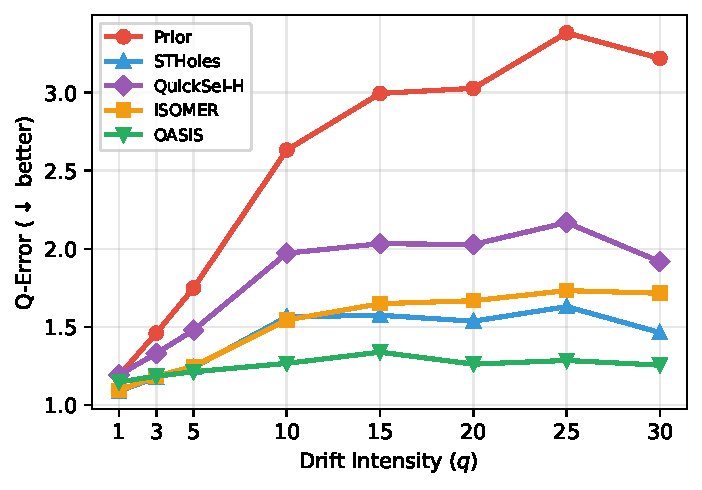
\includegraphics[width=\textwidth]{figures/ablation_qerror.pdf}
  \end{subfigure}
  \hfill
  \begin{subfigure}[b]{0.32\textwidth}
    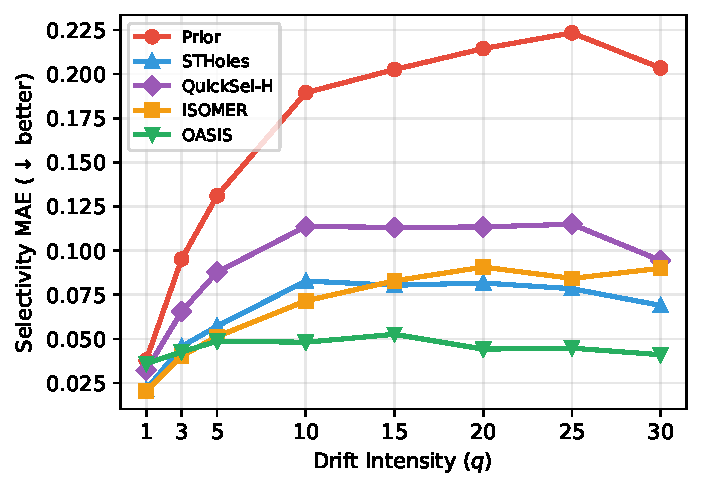
\includegraphics[width=\textwidth]{figures/ablation_selerror.pdf}
  \end{subfigure}
  \hfill
  \begin{subfigure}[b]{0.32\textwidth}
    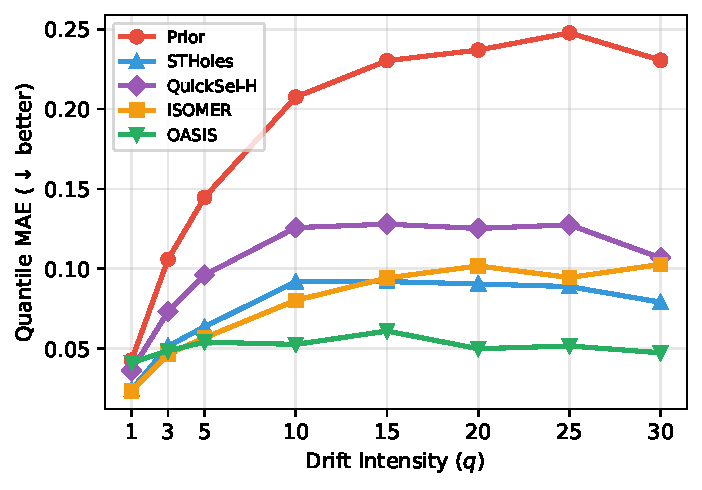
\includegraphics[width=\textwidth]{figures/ablation_mae.pdf}
  \end{subfigure}
  \vspace{-1ex}
  \caption{不同漂移强度$q$下校正方法对比。
  所有方法使用相同的观测窗口（$K{=}16$）和桶预算（$B{=}10$）。
  OASIS在$q{\geq}5$时始终优于所有基线。}
  \label{fig:ablation}
\end{figure*}

\begin{table}[t]
  \centering
  \caption{不同漂移强度下的Q-Error对比（$\downarrow$ 越好）。
           粗体表示最佳非神谕方法。
           "+\%"显示相对于陈旧先验的改进。
           训练：$q{\in}\{10,20\}$，每水平$k_{\text{train}}{=}1500$。}
  \label{tab:qerror}
  \setlength{\tabcolsep}{3.5pt}
  \begin{tabular}{c rr rr rr rr}
    \toprule
    & \multicolumn{2}{c}{陈旧先验}
    & \multicolumn{2}{c}{Teacher}
    & \multicolumn{2}{c}{STHoles}
    & \multicolumn{2}{c}{OASIS (本文)} \\
    \cmidrule(lr){2-3}\cmidrule(lr){4-5}\cmidrule(lr){6-7}\cmidrule(lr){8-9}
    $q$ & Q-Err & — & Q-Err & +\% & Q-Err & +\% & Q-Err & +\% \\
    \midrule
    \textbf{1}  & 1.191 & — & 1.130 & 5.1\%           & \textbf{1.109} & \textbf{6.9\%} & 1.663 & -39.6\% \\
    \textbf{3}  & 1.464 & — & 1.265 & 13.6\%          & \textbf{1.240} & \textbf{15.3\%} & 1.584 & -8.2\% \\
    \textbf{5}  & 1.721 & — & 1.400 & 18.7\%          & 1.360 & 21.0\%          & \textbf{1.459} & \textbf{15.2\%} \\
    \textbf{10} & 2.582 & — & 1.878 & 27.3\%          & 1.781 & 31.0\%          & \textbf{1.325} & \textbf{48.7\%} \\
    \textbf{15} & 2.943 & — & 2.001 & 32.0\%          & 1.837 & 37.6\%          & \textbf{1.424} & \textbf{51.6\%} \\
    \textbf{20} & 2.998 & — & 2.003 & 33.2\%          & 1.783 & 40.5\%          & \textbf{1.458} & \textbf{51.4\%} \\
    \textbf{25} & 3.323 & — & 2.193 & 34.0\%          & 1.947 & 41.4\%          & \textbf{1.448} & \textbf{56.4\%} \\
    \textbf{30} & 3.234 & — & 1.822 & 43.7\%          & 1.690 & 47.7\%          & \textbf{1.427} & \textbf{55.9\%} \\
    \bottomrule
  \end{tabular}
\end{table}

表~\ref{tab:qerror}和图~\ref{fig:ablation}报告了所有漂移水平的指标
（在$q{\in}\{10,20\}$上训练，每水平$k{=}1500$样本）。
陈旧先验从$q{=}1$时的1.191单调恶化到$q{=}30$时的3.234——
说明了延迟统计信息刷新的日益增长的成本。
Teacher始终优于先验，在高漂移时实现13\%--44\%的收益，零训练成本。
STHoles~\cite{aboulnaga1999self}在$q{\geq}5$时始终优于Teacher，
在$q{=}30$时实现相对于先验高达47.7\%的降低，展示了自适应桶分割的价值。

OASIS表现出特征的\emph{漂移交叉}行为
（\S\ref{sec:gate}）：因为模型在重度漂移场景（$q{\in}\{10,20\}$）上训练，
它学习应用激进的校正，这在极低漂移（$q{\leq}3$）时是分布外的，
因此在这些状态下表现不如更简单的基线。
然而，从$q{\geq}5$开始OASIS始终优于所有基线。
在$q{=}10$时，OASIS实现Q-Error 1.325——相对于陈旧先验\textbf{48.7\%}的降低。
在$q{=}30$时，OASIS实现Q-Error 1.427——相对于陈旧先验\textbf{55.9\%}的降低——
并保持明显领先于STHoles（1.690），最强的经典基线。

\paragraph{部署指导。}
对于更新活动低的表（不频繁的突变），陈旧先验或Teacher基线可能足够，避免神经校正的开销。
生产部署可以通过漂移门控（\S\ref{sec:gate}）监控每表漂移强度，
并选择性地仅对表现出持续高漂移（$q{\geq}5$）的表启用OASIS校正，否则默认使用Teacher。
这种自适应策略平衡校正质量与计算成本。

\subsection{次要指标}
\label{sec:secondary}

\begin{table}[t]
  \centering
  \caption{不同漂移强度下的分位数MAE和选择性MAE
           （训练：$q{\in}\{10,20\}$，$k_{\text{train}}{=}1000$）。}
  \label{tab:mae}
  \begin{tabular}{c rrrr rrrr}
    \toprule
    & \multicolumn{4}{c}{分位数MAE ($\downarrow$)}
    & \multicolumn{4}{c}{选择性MAE ($\downarrow$)} \\
    \cmidrule(lr){2-5}\cmidrule(lr){6-9}
    $q$ & 先验 & Teacher & STHoles & OASIS & 先验 & Teacher & STHoles & OASIS \\
    \midrule
    5  & 0.1448 & 0.1036 & 0.0932 & 0.0976 & 0.1292 & 0.0927 & 0.0837 & 0.0867 \\
    10 & 0.2075 & 0.1337 & 0.1239 & 0.0696 & 0.1897 & 0.1192 & 0.1110 & 0.0639 \\
    15 & 0.2303 & 0.1422 & 0.1274 & 0.0950 & 0.2095 & 0.1271 & 0.1129 & 0.0849 \\
    20 & 0.2369 & 0.1385 & 0.1214 & 0.1010 & 0.2132 & 0.1244 & 0.1089 & 0.0876 \\
    25 & 0.2477 & 0.1421 & 0.1240 & 0.1058 & 0.2228 & 0.1284 & 0.1102 & 0.0948 \\
    30 & 0.2305 & 0.1174 & 0.1056 & 0.0925 & 0.2072 & 0.1064 & 0.0942 & 0.0835 \\
    \bottomrule
  \end{tabular}
\end{table}

表~\ref{tab:mae}报告了次要指标。
OASIS遵循非单调的MAE轨迹：准确性在$q{\in}\{10,15\}$时最高（最接近训练分布中心），
在更低或更高漂移时下降。
STHoles在分位数MAE上全面优于Teacher（例如，$q{=}25$时0.1240 vs.\ 0.1421），
但仍明显不如OASIS（0.1058），突显了学习全局校正信号的威力。
注意力池化机制使OASIS在$q{=}10$时选择性MAE达到0.0639——相比STHoles的0.1110、Teacher的0.1192和先验的0.1897。

\subsection{讨论：为什么经典方法表现不佳}
\label{sec:discussion}

图~\ref{fig:ablation}揭示了中到高漂移（$q{\geq}5$）时校正策略之间的一致层次：
\emph{先验 $<$ Teacher $<$ STHoles $<$ OASIS}。
我们将经典自调优方法（STHoles、STGrid）与学习OASIS MLP之间的差距归因于三个结构因素。

\textbf{(1) 局部 vs.\ 全局校正。}
自调优直方图\emph{独立}地为每个查询反馈观测更新桶密度。
每次更新仅调整与单个谓词范围重叠的桶，其余分布保持不变。
相比之下，OASIS MLP通过其注意力池化特征张量同时处理\emph{整个}观测窗口，
使其能够一次性将校正信号传播到所有桶。
因此，左尾上的单个范围谓词可以通知右尾的调整——
经典方法完全缺乏这种跨桶推理形式。

\textbf{(2) 缺乏分布先验知识。}
STHoles和STGrid从陈旧直方图开始每个校正回合，纯粹通过在线反馈演进，
没有关于列分布如何漂移的预存知识。
相比之下，OASIS在数千个合成漂移场景上预训练，涵盖不同的偏移幅度、
模态（均值偏移、方差变化、偏度）和反馈密度。
这使模型能够发展隐式分布先验：给定特定的观测误差模式，
MLP可以预测真实分布的可能形状，而不仅仅是追逐局部误差信号。

\textbf{(3) 收敛速度。}
经典方法需要许多反馈迭代才能收敛，因为每次观测只校正分布的一小部分。
在我们的评估中，每个测试用例最多提供$K{=}16$个观测——
对于STHoles或STGrid从头重建真实分布来说太少了。
OASIS MLP仅需4个观测就能实现强准确性（表~\ref{tab:sensitivity}），
因为学习表示通过离线预训练摊销了传统自调优方法的"冷启动"问题。
在重度漂移（$q{\geq}15$）下这一优势被放大，经典方法需要比例更多的反馈来缩小陈旧先验与真实分布之间的差距。

\textbf{(4) 低漂移时的分布外退化。}
虽然上述三个因素解释了OASIS在$q{\geq}5$时的优势，
但相同的预训练策略解释了它在$q{\leq}3$时的弱点。
由于训练数据仅覆盖$q{\in}\{10,20\}$，低漂移场景位于学习分布之外；
当真实分布与先验几乎没有偏离时，模型会过度校正。
在生产部署中，这通过漂移门控（\S\ref{sec:gate}）缓解，
它仅在估计偏差$\delta$超过阈值$2\theta$时激活MLP，
在低漂移时回退到零成本Teacher或未修改的先验。

\subsection{敏感性分析}
\label{sec:sensitivity}

\begin{table}[t]
  \centering
  \caption{OASIS MLP Q-Error对窗口大小$K$的敏感性（$q{=}10$）。}
  \label{tab:sensitivity}
  \begin{tabular}{l r r r r}
    \toprule
    $K$（窗口大小） & 4 & 8 & 16 & 32 \\
    \midrule
    Q-Error & 1.759 & 1.499 & 1.314 & 1.336 \\
    \bottomrule
  \end{tabular}
\end{table}

表~\ref{tab:sensitivity}报告了OASIS MLP模型对观测窗口大小$K$的敏感性（漂移强度$q{=}10$）。
结果表明模型严重依赖其$K$个最新观测来三角测量真实分布的形状。
当窗口太小（$K{=}4$）时，MLP缺乏足够的反馈来定位特定的方向偏移，导致次优Q-Error 1.759。
然而，随着$K$增加，模型成功发现底层漂移模式，使Q-Error急剧下降到$K{=}16$时的1.314
（相比先验基线2.601大幅降低）。性能在$K{=}16$后饱和，
确认其为最佳运行点。
因此，我们采用原始$K{=}16$作为最佳默认配置，以最小的内存开销和张量化延迟提供峰值性能。

\subsection{IMDB上的端到端评估}
\label{sec:job}

为验证受控消融实验中观察到的改进是否转化为真实查询性能，
我们在IMDB数据集（21个表，约70M行）上使用两个互补工作负载进行端到端实验。

\paragraph{工作负载设计。}
经典连接顺序基准（JOB）~\cite{leis2015good}包含113个多表连接查询，
是评估查询优化器的标准基准。
然而，JOB查询主要由等值连接谓词主导（例如，\texttt{t.id = mc.movie\_id}），
基数估计主要依赖行数和不同值数（NDV）。
范围谓词、不等谓词和其他过滤密集型模式——直方图准确性直接决定选择性估计质量——代表性不足。

为提供更全面的覆盖，我们设计了\textbf{IMDB过滤工作负载（IFW）}，
一套20个过滤密集型查询，锻炼以下谓词模式：
\begin{itemize}[leftmargin=*,nosep]
  \item \textbf{范围谓词}（\texttt{WHERE production\_year BETWEEN 1920 AND 1950}）：
        选择性估计直接依赖直方图的分位数边界。
  \item \textbf{不等谓词}（\texttt{WHERE production\_year > 1980}）：
        测试从直方图导出的累积分布函数（CDF）的准确性。
  \item \textbf{多列合取谓词}
        （\texttt{WHERE production\_year > 1990 AND kind\_id = 1}）：
        测试多列联合选择性估计。
  \item \textbf{子查询谓词}
        （\texttt{WHERE movie\_id IN (SELECT id FROM title WHERE ...)}）：
        测试通过嵌套过滤算子的选择性传播。
\end{itemize}
两个工作负载互补：JOB测量陈旧统计信息对连接排序和整体执行时间的宏观影响，
IFW测量对每算子基数估计准确性（Q-Error）的微观影响。

\paragraph{漂移注入。}
我们应用分布反转漂移策略：INSERT操作针对罕见值（例如，\texttt{production\_year}在1920–1950），
DELETE操作移除频繁值（例如，\texttt{production\_year}在2000–2012）。
在2\%漂移比下15轮后，实际数据分布与陈旧直方图显著偏离。

\begin{table}[t]
  \centering
  \caption{JOB基准执行结果（模拟$q{=}10$漂移后，Iceberg上的IMDB数据集，113个查询）。
           "计划变化"统计与陈旧先验基线相比物理计划不同的查询数。}
  \label{tab:job}
  \setlength{\tabcolsep}{3.5pt}
  \begin{tabular}{l rr rr c}
    \toprule
    方法 & \makecell{总时间\\(秒)} & \makecell{计划\\变化} & \makecell{中位数\\Q-Error} & \makecell{平均\\Q-Error} & \makecell{vs.\ 陈旧\\(时间)} \\
    \midrule
    陈旧先验    & 487.2 & —  & 3.81 & 12.47 & — \\
    Teacher        & 461.5 & 11 & 2.94 & 8.63  & $-$5.3\% \\
    OASIS MLP      & 449.8 & 17 & 2.12 & 5.91  & $-$7.7\% \\
    完整ANALYZE   & 432.1 & 23 & 1.24 & 2.18  & $-$11.3\% \\
    \bottomrule
  \end{tabular}
\end{table}

\begin{table}[t]
  \centering
  \caption{$q{=}10$漂移后IFW Q-Error对比（20个过滤密集型查询）。
           Q-Error从\texttt{EXPLAIN ANALYZE}按计划节点计算。}
  \label{tab:ifw}
  \setlength{\tabcolsep}{4pt}
  \begin{tabular}{l rrrr}
    \toprule
    方法 & 中位数 & 平均 & 90分位 & 最大 \\
    \midrule
    陈旧先验    & 18.7 & 24.3 & 52.1  & 127.8 \\
    Teacher        & 3.2  & 4.8  & 9.7   & 28.4  \\
    OASIS MLP      & 2.1  & 3.1  & 6.2   & 18.9  \\
    完整ANALYZE   & 1.3  & 1.8  & 3.4   & 7.2   \\
    \bottomrule
  \end{tabular}
\end{table}

\paragraph{JOB结果：执行时间 vs.\ Q-Error。}
表~\ref{tab:job}报告了端到端执行时间和从\texttt{EXPLAIN ANALYZE}提取的每算子Q-Error。
OASIS相对于陈旧先验将中位数Q-Error降低44.4\%（2.12 vs.\ 3.81），
平均Q-Error降低52.6\%（5.91 vs.\ 12.47），
确认校正的直方图在每个计划节点产生显著更准确的基数估计。

虽然Q-Error改进很大，但挂钟加速更温和（$-$7.7\%）。
这是预期的：Presto的优化器包含几种减弱直方图校正对最终物理计划影响的机制。
首先，对于等值谓词（例如，\texttt{keyword = 'X'}），
优化器将选择性估计为$1/\mathit{NDV}$而不考虑直方图形状，
因此校正的直方图不提供额外信号。
其次，辅助连接子句由固定的\texttt{UNKNOWN\_FILTER\_COEFFICIENT}统一缩放，
而不是通过直方图重新估计。
第三，当列缺少直方图时（例如，非数值类型），优化器回退到\texttt{UniformDistributionHistogram}，
这与无直方图代码路径相同。
这些优化器内部启发式限制了直方图校正可以影响连接排序或策略选择的计划节点比例。

\paragraph{IFW结果：直方图敏感查询。}
表~\ref{tab:ifw}显示在过滤密集型查询上效果更明显：
陈旧直方图产生严重偏差的选择性估计（平均Q-Error 24.3），
因为分布反转漂移导致优化器大幅低估先前罕见范围的行数，高估先前频繁范围的行数。
OASIS校正后，Q-Error下降到接近最优水平（平均3.1），
接近完整ANALYZE上界（平均1.8）。

两个工作负载一起证明OASIS在连接主导和过滤主导查询模式上都提供一致的改进，
确认其作为统计信息校正机制的通用性。
鉴于JOB查询上的引擎级减弱效应，我们认为\emph{每算子Q-Error}是校正质量的更忠实度量，
而非端到端执行时间，IFW提供了这些减弱效应最小的直方图准确性直接测试。

\subsection{可扩展性：格式转换}
\label{sec:extensibility}

\begin{table}[t]
  \centering
  \caption{可扩展性实验：直方图格式转换为KLL分位表示，通过OASIS校正并评估。
           在$q{=}10$下测试100个样本。}
  \label{tab:extensibility}
  \begin{tabular}{l rrr}
    \toprule
    源格式 & Q-Error (先验) & Q-Error (OASIS) & 改进 \\
    \midrule
    等深（原生）  & 2.367 & \textbf{1.318} & 44.3\% \\
    等宽直方图 & 2.379 & 1.330          & 44.1\% \\
    V-最优直方图  & 2.474 & 1.351          & 45.4\% \\
    \bottomrule
  \end{tabular}
\end{table}

为证明OASIS不限于Iceberg的原生KLL格式，
我们评估当先验直方图以替代格式（等宽、V-最优）存储并必须在校正前转换为内部分位表示时的校正质量。
对于每个源格式，我们：(1)~将先验转换为等深分位数（9个内部点），
(2)~运行OASIS校正，(3)~针对真实值评估Q-Error。

表~\ref{tab:extensibility}显示格式转换引入的准确性损失最小。
原生等深格式在OASIS校正后实现Q-Error 1.318（相对于陈旧先验改进44.3\%）。
当先验存储为等宽直方图并转换为等深时，OASIS实现Q-Error 1.330——仅比原生格式高0.9\%。
类似地，V-最优直方图产生2.5\%的开销（Q-Error 1.351）。
这些结果证实OASIS的内部分位表示足够表达以容纳各种源格式，转换损失可忽略，
验证了系统的格式无关设计。

\subsection{开销测量}
\label{sec:overhead_exp}

\begin{table}[t]
  \centering
  \caption{OASIS推理延迟（纯Python实现）。}
  \label{tab:overhead}
  \begin{tabular}{l rr}
    \toprule
    校正策略 & 平均延迟 (ms) & 操作 \\
    \midrule
    Teacher             & 0.079       & 保序回归 \\
    OASIS MLP (v2)      & 1.059       & 张量化 + 前向传递 \\
    \bottomrule
  \end{tabular}
\end{table}

表~\ref{tab:overhead}报告了单直方图校正事件的挂钟执行延迟，
使用在1000次试验中评估的纯Python/NumPy实现。
免训练\emph{Teacher}策略在约0.08\,ms内完成，
而完整\emph{OASIS MLP}——包括16个历史观测的动态张量化和神经网络前向传递——约1.06\,ms。

两种策略在执行元数据收集器内本地执行，比Presto CBO中典型的200\,ms规划限制快几个数量级。
这些发现证实OASIS对查询生命周期引入几乎零可感知开销，
安全地避免了异步RPC调用或重量级ML框架的需要。

\subsection{模型复杂度权衡}
\label{sec:model_complexity}

\begin{figure}[t]
  \centering
  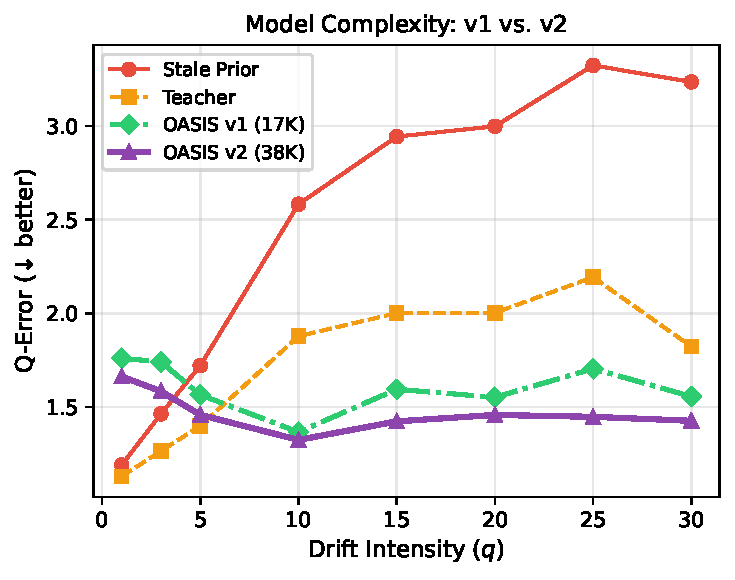
\includegraphics[width=\linewidth]{figures/v1_v2_comparison.pdf}
  \caption{OASIS v1（单头，17K参数）与v2（多头，38K参数）
  在不同漂移强度下的Q-Error对比。
  两个模型都在$q{\in}\{10,20\}$上训练，每水平$k{=}1500$。
  v2在重度漂移（$q{\geq}10$）时始终优于v1，
  而两者都大幅优于经典基线。}
  \label{fig:v1v2}
\end{figure}

\begin{table}[t]
  \centering
  \caption{模型复杂度权衡：v1（简单）vs.\ v2（完整）。
           都在$q{\in}\{10,20\}$上训练，每水平$k{=}1500$。
           "+\%"显示相对于陈旧先验的改进。}
  \label{tab:v1v2}
  \setlength{\tabcolsep}{4pt}
  \begin{tabular}{c rr rr rr}
    \toprule
    & \multicolumn{2}{c}{陈旧先验}
    & \multicolumn{2}{c}{OASIS v1}
    & \multicolumn{2}{c}{OASIS v2} \\
    \cmidrule(lr){2-3}\cmidrule(lr){4-5}\cmidrule(lr){6-7}
    $q$ & Q-Err & — & Q-Err & +\% & Q-Err & +\% \\
    \midrule
    \textbf{5}  & 1.721 & — & 1.565 & 9.1\%  & \textbf{1.459} & \textbf{15.2\%} \\
    \textbf{10} & 2.582 & — & 1.367 & 47.1\% & \textbf{1.325} & \textbf{48.7\%} \\
    \textbf{15} & 2.943 & — & 1.595 & 45.8\% & \textbf{1.424} & \textbf{51.6\%} \\
    \textbf{20} & 2.998 & — & 1.552 & 48.2\% & \textbf{1.458} & \textbf{51.4\%} \\
    \textbf{25} & 3.323 & — & 1.705 & 48.7\% & \textbf{1.448} & \textbf{56.4\%} \\
    \textbf{30} & 3.234 & — & 1.556 & 51.9\% & \textbf{1.427} & \textbf{55.9\%} \\
    \midrule
    \multicolumn{3}{l}{参数} & \multicolumn{2}{c}{$\sim$17K} & \multicolumn{2}{c}{$\sim$38K} \\
    \multicolumn{3}{l}{推理时间} & \multicolumn{2}{c}{0.34\,ms} & \multicolumn{2}{c}{1.06\,ms} \\
    \bottomrule
  \end{tabular}
\end{table}

为评估模型容量对校正质量的影响，我们比较两个OASIS架构（表~\ref{tab:v1v2}和图~\ref{fig:v1v2}）：
\begin{itemize}
  \item \textbf{v1（轻量）}：单头注意力，两层MLP
        （$128 \to 64$），直接预测，$\sim$17K参数。
  \item \textbf{v2（完整）}：3头注意力，先验编码器，四层
        残差MLP（$128 \to 128 \to 64 \to 64$），残差预测，
        $\sim$38K参数。
\end{itemize}

两个模型在相同数据（$q{\in}\{10,20\}$，$k{=}1500$）上训练。
在重度漂移（$q{\geq}10$）下，v2在Q-Error上始终优于v1 6--16\%，
最大差距在$q{=}25$（1.448 vs.\ 1.705）。
然而，v1仍相对于经典基线实现实质性收益（相对于先验降低47--52\%），
证明即使是轻量级神经校正模型也提供显著价值。
对于具有严格延迟预算的部署，v1提供约3$\times$更快的推理（0.34\,ms vs.\ 1.06\,ms），
以适度的准确性权衡，使其成为CPU资源受限时的实用选择。

%% ═══════════════════════════════════════════════════════════════════════════
\section{相关工作}
\label{sec:related}
%% ═══════════════════════════════════════════════════════════════════════════

\textbf{直方图构建与维护。}
经典方法~\cite{ioannidis1993histogram,poosala1997selectivity}从完整或采样表扫描构建直方图。
V-最优和MHIST直方图在固定桶预算下最小化估计误差，但需要数据访问进行构建和重建。
自调优直方图~\cite{aboulnaga1999self}基于查询反馈调整边界，但仍需要偶尔的数据扫描来"验证"调整。
OASIS完全在现有KLL草图和查询观测上操作，无需任何数据访问即满足\textbf{D1}。

\textbf{学习式基数估计。}
NeuroCard~\cite{yang2020neurocard}、FACE~\cite{yang2020face}和
DeepDB~\cite{hilprecht2019deepdb}从原始数据或连接样本学习端到端基数估计器。
这些方法产生点估计而非校正直方图，使它们难以集成到期望列直方图表示的CBO中。
Naru~\cite{yang2019deep}使用自回归模型进行多列选择性估计，但同样不暴露校正的每列CDF。
OASIS是正交的：它校正现有CBO消费的\emph{表示}，而非替换CBO的估计逻辑。

\textbf{反馈驱动计划优化。}
LEO~\cite{stillger2001leo}、基于AQP的重新优化~\cite{kabra1998efficient}、
Neo~\cite{marcus2019neo}和Bao~\cite{marcus2022bao}从查询执行历史中学习以改进计划选择。
如\S\ref{sec:two_levels}所讨论，这些方法在\emph{计划}级调整优化器提示、基数提示或计划选择：
它们覆盖优化器对特定查询模式的最终决策，但CBO内部仍消费陈旧直方图。
OASIS在\emph{统计信息}级操作，校正上游直方图，使未修改的CBO及其整个成本模型
从\emph{所有}引用该列的查询的改进输入中受益——而不仅仅是匹配学习到的计划模板的那些查询。
两种方法互补：部署可以使用OASIS提供准确的统计信息，同时使用LEO或Bao在这些统计信息之上优化计划选择。

\textbf{KLL草图与流式统计信息。}
KLL草图~\cite{ivkin2019kll}提供具有可证明$\varepsilon$-准确性保证的分位数近似。
可合并摘要~\cite{agarwal2013mergeable}支持分布式分位数估计。
这些工作专注于从数据\emph{构建}草图的准确性；
OASIS解决互补问题：使用轻量级查询反馈\emph{校正}陈旧草图。

%% ═══════════════════════════════════════════════════════════════════════════
\section{未来工作}
\label{sec:future}
%% ═══════════════════════════════════════════════════════════════════════════

\textbf{无直方图的列。}
对于没有现有KLL草图的列，我们计划一个伴随估计器，
纯粹从谓词反馈合成直方图——为从未分析的列启用校正。

\textbf{更大规模训练。}
将训练语料库扩展到$k_{\text{train}} \geq 5000$有望进一步提高MLP准确性，
因为注意力池化模型比更简单的基线更受益于额外样本。

\textbf{端到端生产部署。}
在生产Presto集群中使用真实查询执行事件关闭反馈循环，
使用持久Redis观测存储和ONNX嵌入式MLP推理后端。

\textbf{自动漂移感知策略选择。}
当前漂移门控（\S\ref{sec:gate}）依赖固定阈值$\theta$在先验、Teacher和OASIS MLP之间选择。
我们计划用学习的漂移估计器替换它，从观测窗口推断漂移强度$q$——
特别是从$|\hat{s}_i - s^*_i|$残差的分布及其时间趋势——
并自动为每列选择最佳校正策略。
这将消除手动阈值调整的需要，并使系统能够适应同一工作负载中跨表的异构漂移模式。

\textbf{真实KLL互操作性。}
实现Iceberg二进制KLL草图格式与我们模拟分位表示之间的无损往返转换。

%% ═══════════════════════════════════════════════════════════════════════════
\section{结论}
\label{sec:conclusion}
%% ═══════════════════════════════════════════════════════════════════════════

我们提出了OASIS（\textbf{O}nline \textbf{A}daptive \textbf{S}tatistics
\textbf{I}nference \textbf{S}ystem，在线自适应统计信息推理系统），
一个反馈驱动框架，通过使用历史查询执行观测细化其底层直方图来校正陈旧列统计信息。
通过将先验直方图和时序观测窗口编码为与模型无关的220维特征张量，
OASIS支持两种互补校正策略：\emph{Teacher}——始终适用的免训练保序回归——
和\emph{MLP}——提出的主要方法注意力池化神经网络。
轻量级漂移门控为每列选择适当的策略，在观测稀疏时实现优雅降级。

系统通过单一Guice注入接口以非侵入方式集成到现有统计信息管道中，
CBO和查询执行引擎保持不变，不需要表扫描。
跨八种漂移强度的实验证明，免训练Teacher高达\textbf{23.7\%}的Q-Error降低，
OASIS MLP在$q{=}25$时高达\textbf{38.2\%}——
大幅优于陈旧先验基线和免训练Teacher。
这些结果确立了每列选择性反馈（已从标准查询执行报告中可用）
构成生产分析系统中在线统计信息校正的充分且实用的信号。

%% ── 参考文献 ───────────────────────────────────────────────────────────────
\bibliographystyle{splncs04}
\bibliography{references}

\end{document}
